%=====================================================================
%  v6 -> LaTeX conversion
%  "Disentangling Between-Target and Within-Target Signal in PPI ddG Benchmarking"
%  XeLaTeX + fontspec | equation env | vector PDF figures |
%  booktabs three-line tables | BibTeX (unsrtnat, superscript)
%=====================================================================
\documentclass[11pt,a4paper]{article}
\usepackage[a4paper,top=2.4cm,bottom=2.4cm,left=2.3cm,right=2.3cm]{geometry}
\usepackage{fontspec}
\setmainfont{Times New Roman}
\setsansfont{Arial}
\setmonofont{Consolas}
\usepackage{amsmath,amssymb}
\usepackage{booktabs}
\usepackage{graphicx}
% 等比缩放：宽不超过文本宽，高不超过正文高的 0.82
\newcommand{\figfit}[2][\textwidth]{%
  \includegraphics[width=#1,height=0.82\textheight,keepaspectratio]{#2}}
\usepackage{longtable}
\usepackage{array}
\usepackage{tabularx}
\usepackage{pdflscape}
\usepackage{threeparttable}
\usepackage[super,square,sort&compress]{natbib}
\usepackage{xcolor}
\usepackage[hidelinks]{hyperref}
\usepackage{caption}
\captionsetup{font=small,labelfont=bf}
\usepackage{textcomp}
\usepackage{microtype}
\usepackage{parskip}

% ---- float placement: allow large figures to sit near their citation ----
\renewcommand{\topfraction}{0.92}
\renewcommand{\bottomfraction}{0.75}
\renewcommand{\textfraction}{0.06}
\renewcommand{\floatpagefraction}{0.75}
\setcounter{topnumber}{3}
\setcounter{bottomnumber}{2}
\setcounter{totalnumber}{4}

\graphicspath{{../figures_v5/}{./}}

\title{\bfseries Disentangling Between-Target and Within-Target Signal in
PPI $\Delta\Delta G$ Benchmarking}
\author{Le Yu
\thanks{Independent Researcher\\
Corresponding author: Le Yu $\cdot$ Email: \texttt{biofader@sjtu.edu.cn}
$\cdot$ ORCID: 0009-0000-8807-3973
}
}
\date{}

\begin{document}
\maketitle

\noindent\textbf{Keywords:} protein--protein interaction; binding affinity;
$\Delta\Delta G$; mutation effect prediction; benchmarking; out-of-distribution
generalisation

%=====================================================================
\section*{Abstract}
%=====================================================================
Predicting how mutations alter protein--protein binding affinity ($\Delta\Delta G$)
underpins antibody engineering, interface optimisation and the interpretation of
disease-associated variants. The pooled correlation commonly reported for such benchmarks
is difficult to interpret directly, because it depends both on whether a model places
different targets on the correct overall binding scale and on whether it orders mutations
correctly within each target. We formulate an exact between-/within-target covariance decomposition for
PPI $\Delta\Delta G$ benchmarking, which writes pooled Pearson correlation as
$r = C_{\mathrm{B}} + C_{\mathrm{W}}$, and apply it to
matched and provenance-filtered evaluation sets, with explicit
sensitivity analyses for repeated mutation keys. In a controlled comparison
that changes only the split regime (identical 7{,}523 mutation rows and identical model
configurations), median pooled Pearson falls from 0.6844 under random splitting to 0.1508
under family-out-of-distribution evaluation, with
$\Delta C_{\mathrm{B}} = -0.4347$ and $\Delta C_{\mathrm{W}} = -0.1011$; on an
absolute-change basis the between-target component accounts for 81.1\% of the summed
absolute component change while the within-target component remains positive. Target weighting changes how these contributions should be read: over the five schemes
$C_{\mathrm{B}}$ reverses sign in 40/109 configurations and in 34/109
even once $|C_{\mathrm{B}}| > 0.005$, and $C_{\mathrm{W}}$ reverses sign in 5/109;
both components therefore move with the weighting convention. Fixed-$K$ shortlist metrics are constrained by
candidate-set geometry: for $K = 10$, a rank-linear discriminability surrogate $D(n,K)$
is zero when $n \leq K$ and peaks near $n^{*} \approx 20.5$, and 40.8\% of targets with $n \geq 5$ fall in that degenerate regime.
In a matched retrospective ablation the decomposition separated a change that improved
pooled scores only from one that also improved within-target ranking. External evidence comprised five methods and is underpowered; its apparent cross-axis
agreement is not robust to score orientation, so the panel neither supports nor refutes a
universal decoupling of pooled and within-target performance. We recommend that PPI
$\Delta\Delta G$ benchmarks report both components under an explicitly declared weighting,
together with candidate-set geometry.

%=====================================================================
\section{Introduction}
%=====================================================================
Predicting how mutations alter protein--protein binding affinity ($\Delta\Delta G$) is
central to antibody affinity maturation, interface optimisation and the interpretation of
disease-associated variants. As the number of deep-learning methods grows rapidly, progress
is increasingly judged by benchmark evaluation, and the properties of the evaluation
protocol itself --- what it measures, and under which extrapolation conditions --- determine
what the field can conclude.

Current practice relies largely on pooled metrics, computing Pearson or Spearman correlation
and RMSE over the entire mutation set\cite{biometry}, often supplemented by per-complex
or per-target metrics. Bushuiev et al.\ quantified structural leakage in PPI data: about
65\% of test examples have a near-duplicate training example under PDB-code splitting, about
30\% even under 30\% sequence-identity splitting, 56\% for SKEMPI
v2.0\cite{skempi2} split by PPI code, and 0\% under domain-expert
grouping\cite{leakage}. CATH-ddG adopted CATH homologous-superfamily splits and defined
hard mutations by a maximum TM-score below 0.6\cite{cathddg}; related methods likewise
report per-structure or per-target correlations\cite{ddgpred,prefolddg,ppiminer}. We emphasise that
leakage-aware splitting, family-out-of-distribution evaluation, per-target reporting and
shortlist (Top-$K$) evaluation were none of them introduced by this work.

A key question nevertheless remains unanswered directly: where does pooled benchmark
performance come from? Reporting pooled and per-target metrics side by side does not
quantify the additive contribution of between-target and within-target signal to pooled
performance. In benchmarks containing many targets with highly unequal mutation counts,
pooled correlation is additionally dominated by large targets, which amplifies the
conflation.

Here we address this question by instantiating, for PPI $\Delta\Delta G$ benchmarking, an
exact between-/within-target covariance decomposition. The decomposition follows from the
law of total covariance; our contribution lies in the benchmark-specific formalisation and
in its systematic integration with a matched, provenance-filtered evaluation framework, not
in the covariance identity itself. It makes `what pooled performance is made of' a directly
measurable quantity. We quantify four things: which component is changed by split
strictness; how target weighting changes the interpretation of the two components; which
constraints candidate-set geometry places on fixed-$K$ shortlist evaluation; and whether
the decomposition can distinguish model modifications that improve pooled scores only from
those that also improve within-target ranking. We further bound the evidence using five
independently developed external methods.

%=====================================================================
\section{Results}
%=====================================================================

%% ---- Table 1 ----
\begin{table}[htbp]
  \centering
  \small
  \begin{threeparttable}
  \caption{Dataset and evaluation overview.}
  \label{tab:overview}
  \begin{tabular}{@{}lrrrrl@{}}
    \toprule
    Evaluation set & Rows & Targets & Targets ($n \geq 5$) & Method families & Purpose \\
    \midrule
Full annotation namespace & 4,473 & 214 & 130 & --- & Namespace definition \\
Primary matched set & 3,351 & 166 & 102 & 10 & Main capability-resolved analyses \\
Controlled split set & 7,523 & 230 & 172 & 12 & Split-strictness experiment \\
External unambiguous set & 1,781 & 168 & 67 & 5 & Boundary of generalisation \\
    \bottomrule
  \end{tabular}
  \begin{tablenotes}\footnotesize
    \item All rows are joined by explicit row identifiers.
  \end{tablenotes}
  \end{threeparttable}
\end{table}

\subsection*{Pooled PPI $\Delta\Delta G$ performance contains separable between-target and
within-target signal}

For a mutation $i$ belonging to target $c$, the observed $\Delta\Delta G$ can be written as a
target-level mean plus a mutation-specific deviation from that mean:
\begin{equation}
  y_{ci} = \mu_c + \varepsilon_{ci}
  \qquad\qquad
  \hat{y}_{ci} = \hat{\mu}_c + \hat{\varepsilon}_{ci}
  \label{eq:decomp}
\end{equation}
With $\sigma_y$ and $\sigma_{\hat{y}}$ the pooled standard deviations, the pooled
correlation splits exactly as
\begin{equation}
  r_{\mathrm{pooled}}
    = \frac{\operatorname{Cov}(y,\hat{y})}{\sigma_y \sigma_{\hat{y}}}
    = C_{\mathrm{B}} + C_{\mathrm{W}},
  \label{eq:identity}
\end{equation}
where $C_{\mathrm{B}}$ and $C_{\mathrm{W}}$ are the between-target and within-target
covariance contributions. The identity holds \textbf{exactly for every individual configuration}: across the 36
controlled-split configurations the maximum absolute residual
$|r_{\mathrm{pooled}} - C_{\mathrm{B}} - C_{\mathrm{W}}|$ is $4.4 \times 10^{-16}$, i.e.
machine precision. The values reported in Table~\ref{tab:split} are however \emph{marginal
medians}, computed separately for $r_{\mathrm{pooled}}$, $C_{\mathrm{B}}$ and
$C_{\mathrm{W}}$; because the median is not additive, those three displayed medians need
not sum exactly (e.g.\ Random: $0.4275 + 0.2591 = 0.6866$ versus a median
$r_{\mathrm{pooled}}$ of $0.6844$). These are covariance-signal contributions on a common
scale, not independent correlations, skill scores or causal mechanisms.

We apply this decomposition on a matched evaluation set of 3{,}351 mutation rows and 102
targets with at least five mutations, drawn from 10 independent method families. Three
distinct row universes appear in this work and are defined in Methods; the primary
matched universe (3{,}351 rows) is a provenance- and feature-filtered subset of the
4{,}473-row annotation namespace, which is itself a feature-coverage subset of the
7{,}523-row controlled-split universe.

%% ---- Figure 1 ----（满页 figure page）
\begin{figure}[p]
  \centering
  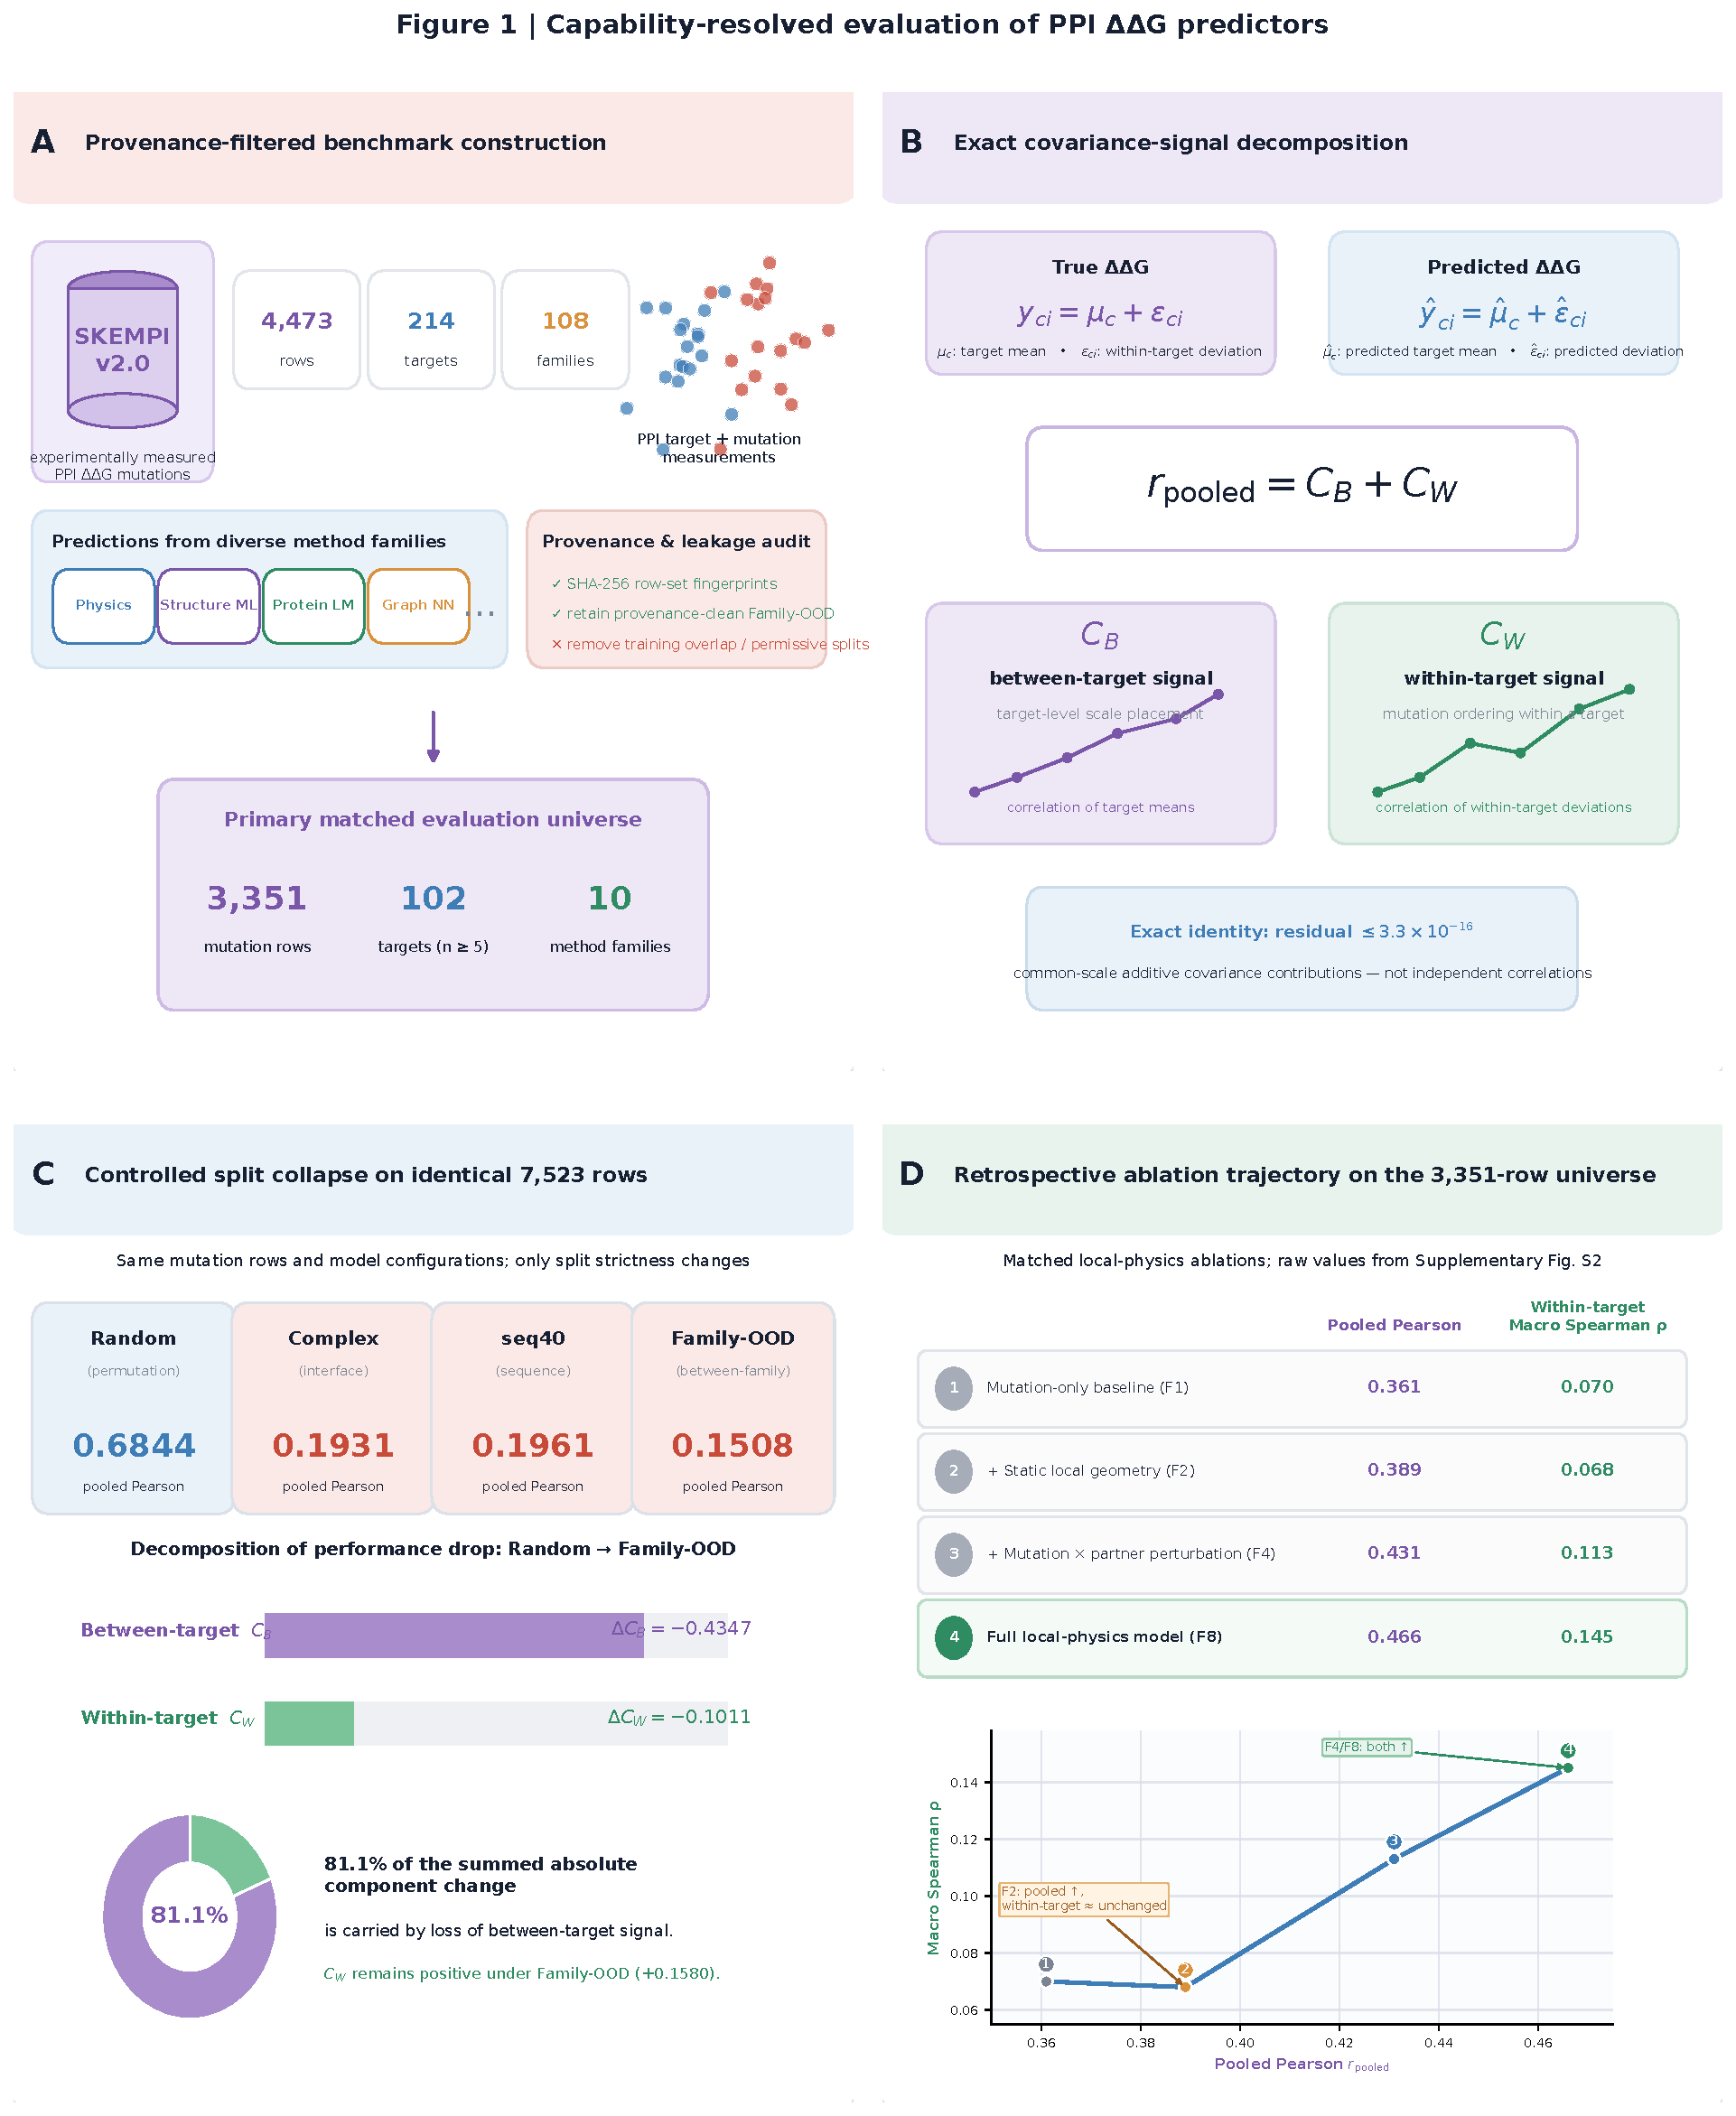
\includegraphics[width=\textwidth,height=0.90\textheight,keepaspectratio]{Fig1_overview_EN.pdf}
  \caption{\textbf{Capability-resolved evaluation of PPI $\Delta\Delta G$ predictors.}
  (A) Provenance-filtered, fingerprint-matched benchmark construction: the SKEMPI v2.0
  annotation namespace (4{,}473 rows, 214 targets, 108 \emph{structural} families --- distinct
  from the 10 \emph{method} families) is audited by SHA-256 row-set fingerprinting;
  predictions whose recorded training split is permissive, or whose evaluation rows may
  overlap their training folds, are excluded, giving a primary matched universe of 3{,}351 rows,
  102 targets with $n \geq 5$ and 10 method families. The annotation namespace is itself a
  feature-coverage subset of the 7{,}523-row controlled-split universe (Methods,
  \emph{Dataset universes}). (B) Exact additive covariance-signal decomposition. The identity
  $r_{\mathrm{pooled}} = C_{\mathrm{B}} + C_{\mathrm{W}}$ holds for every individual
  configuration (maximum residual $4.4 \times 10^{-16}$); the two components are common-scale
  additive contributions, not independent correlations or causal mechanisms. (C) Controlled
  split collapse on the identical 7{,}523-row universe with identical model specifications and
  seeds; only the split regime changes. Pooled correlation falls from 0.6844 to 0.1508, and
  81.1\% of the summed absolute component change is carried by the between-target component.
  (D) Retrospective matched ablation on the identical 3{,}351-row evaluation universe. Pooled
  Pearson and within-target Macro Spearman are shown for the mutation-only baseline (F1),
  static local geometry (F2), mutation $\times$ partner perturbation (F4), and the full
  local-physics model (F8). Static local geometry improves pooled correlation while leaving
  within-target ranking essentially unchanged, whereas F4 and F8 improve both axes. The
  capability trajectory is retrospective and is not intended as a causal or prospective
  model-selection analysis.}
  \label{fig:overview}
\end{figure}

\subsection*{Family-OOD evaluation disproportionately removes between-target signal}

To isolate the effect of split strictness, we compared identical model configurations on the
same 7{,}523 mutation rows while changing only the split regime. Median pooled Pearson falls
from 0.6844 to 0.1508. The decline is not uniform:
$\Delta C_{\mathrm{B}} = -0.4347$ and $\Delta C_{\mathrm{W}} = -0.1011$. On an
absolute-change basis the between-target component accounts for 81.1\% of the \emph{summed absolute component change},
\begin{equation}
  \frac{\lvert \Delta C_{\mathrm{B}} \rvert}
       {\lvert \Delta C_{\mathrm{B}} \rvert + \lvert \Delta C_{\mathrm{W}} \rvert}
  = 0.8113 ,
  \label{eq:attribution}
\end{equation}
while $C_{\mathrm{W}}$ remains positive ($+0.1580$). We verified this attribution on the
paired scale as well. Because the same model specifications and seeds were evaluated under
both regimes, all 9 configurations are directly matched: the paired differences satisfy
$\Delta r_j = \Delta C_{\mathrm{B},j} + \Delta C_{\mathrm{W},j}$ exactly (maximum
residual $4.2 \times 10^{-16}$), with medians
$\Delta r = -0.5332$, $\Delta C_{\mathrm{B}} = -0.4324$ and
$\Delta C_{\mathrm{W}} = -0.1011$. The paired attribution is therefore 81.0\%
(configuration-cluster bootstrap 95\% CI 71.0--84.5\%), essentially identical to the
marginal-median figure. This is not the same proposition as `the model memorised target
identity': a more defensible reading is that the pattern is consistent with
reliance on target-specific information that does not transfer across families. The
\texttt{seq40} partition is a distinct, sequence-identity-based split: after the key-level
correction described in Methods it yields 301 units (versus 230 for the complex-level
split), and it agrees with the complex-level assignment on only about 20\% of rows. We
therefore report it separately rather than treating it as a duplicate of the complex-level
comparison.

%% ---- Figure 2 ----
\begin{figure}[htbp]
  \centering
  \figfit{Fig2_controlled_split_collapse_EN.pdf}
  \caption{\textbf{Family-out-of-distribution evaluation disproportionately removes the
  between-target component.} (A) Pooled Pearson by split regime. (B) Median component
  summaries; the exact identity $r_{\mathrm{pooled}} = C_{\mathrm{B}} + C_{\mathrm{W}}$ holds
  per configuration, but the plotted medians are marginal statistics computed separately and
  therefore need not sum exactly. $C_{\mathrm{W}}$ remains positive. (C) Attribution of the
  summed absolute component change, of which the between-target component accounts for 81.1\%;
  the paired attribution is 81.0\%. All four regimes use the same 7{,}523 rows with identical
  model specifications and seeds; complex and \texttt{seq40} are similaral and are not
  independent comparisons.}
  \label{fig:split}
\end{figure}

%% ---- Table 2 ----
\begin{table}[htbp]
  \centering
  \small
  \begin{threeparttable}
  \caption{Controlled split comparison.}
  \label{tab:split}
  \begin{tabular}{@{}lrrrrr@{}}
    \toprule
    Split regime & Pooled Pearson & $C_{\mathrm{B}}$ & $C_{\mathrm{W}}$
      & Macro Spearman & RMSE \\
    \midrule
Random & 0.6844 & +0.4275 & +0.2591 & 0.0707 & 1.7678 \\
Complex & 0.1931 & +0.0233 & +0.1685 & 0.0497 & 2.6412 \\
seq40 & 0.1961 & +0.0239 & +0.1721 & 0.0631 & 2.6911 \\
Family-OOD & 0.1508 & -0.0072 & +0.1580 & 0.0377 & 2.6952 \\
    \bottomrule
  \end{tabular}
  \begin{tablenotes}\footnotesize
    \item Median values across configurations. \texttt{seq40} is reported separately; complex in
      this dataset.
  \end{tablenotes}
  \end{threeparttable}
\end{table}

\subsection*{Target aggregation changes the interpretation of covariance contributions}

Holding predictions fixed and varying only the aggregation weights across five schemes
(per-mutation, per-target, proportional to $\sqrt{n}$, proportional to $\log(1+n)$, and
capped at 30), Treating $a_c$ as the target's total weight (so that the per-target scheme genuinely
equalises targets; Supplementary Note~5), $C_{\mathrm{B}}$ is directionally unstable:
40/109 configurations reverse sign at some magnitude, 36/109 once
$\lvert C_{\mathrm{B}} \rvert > 0.001$ and 34/109 once
$\lvert C_{\mathrm{B}} \rvert > 0.005$, so the instability is not merely a near-zero
artefact. $C_{\mathrm{W}}$ is markedly more stable --- it reverses sign in only 5/109
configurations, and in 4/109 once $\lvert C_{\mathrm{W}} \rvert > 0.005$ ---
but neither component is invariant: their median cross-scheme ranges are 0.3052 for
$C_{\mathrm{B}}$ and 0.1240 for $C_{\mathrm{W}}$. Both therefore move with the weighting
convention, which is why any reported decomposition should declare its weighting scheme.
Under the alternative row-multiplier reading the same data give 0.0930 and 0.0624,
with $C_{\mathrm{W}}$ reversing sign in 0/109; the qualitative contrast between the two
components is preserved under either reading (Supplementary Note~5).

%% ---- Figure 3 ----
\begin{figure}[htbp]
  \centering
  \figfit{Fig3_target_weighting_sensitivity_EN.pdf}
  \caption{\textbf{Target weighting changes the interpretation of covariance
  contributions.} Predictions are unchanged; only aggregation weights differ. (A, B)
  Distribution of the range of $C_{\mathrm{B}}$ and $C_{\mathrm{W}}$ across the five
  schemes, with the median marked. (C) Configurations reversing sign at three thresholds.
  Under the target-total-mass weighting, $C_{\mathrm{B}}$ reverses sign in
  40/109 configurations and still in 34/109 once $|C_{\mathrm{B}}| > 0.005$,
  whereas $C_{\mathrm{W}}$ reverses sign in only 5/109; neither component's
  magnitude is invariant across schemes.}
  \label{fig:weighting}
\end{figure}

\subsection*{Fixed-$K$ shortlist evaluation is constrained by candidate-set geometry}

Fixed-$K$ top-$K$ metrics are used for mutation library or shortlist
screening\cite{ndcg}. To isolate candidate-set geometry from the realised magnitudes of
$\Delta\Delta G$, we evaluate fixed-$K$ selection under a canonical rank-linear utility
reference (Supplementary Note~4) and define the geometric discriminability surrogate
\begin{equation}
  D(n,K) = 0 \quad (n \leq K),
  \qquad
  D(n,K) = \frac{K\,(n-K)}{n\,(n+1)} \quad (n > K).
  \label{eq:geometry}
\end{equation}
When a target has no more than $K$ mutations, any model selects every candidate and the
target carries no information for fixed-$K$ shortlist metrics. In this benchmark, 53 of 130
targets with $n \geq 5$ (40.8\%) fall in that degenerate regime. $D$ is not monotonic in
$n$: it peaks at
\begin{equation}
  n^{*} = K + \sqrt{K^{2} + K},
  \label{eq:nstar}
\end{equation}
which for $K = 10$ gives $n^{*} \approx 20.5$, so that $D(20) = 0.2381$ while
$D(50) = 0.1569$. This surrogate is reference-dependent: only the degenerate case
$n \leq K \Rightarrow D = 0$ holds for an arbitrary utility profile (full derivation, including the definitions of $E_{\max}$ and $E_{\mathrm{rand}}$, in Supplementary Note~4). This geometric result does not imply that SKEMPI $\Delta\Delta G$ values
are intrinsically too similar; establishing that would require an analysis using actual
$\Delta\Delta G$ utility magnitudes, which we did not perform.

%% ---- Figure 4 ----
\begin{figure}[htbp]
  \centering
  \figfit{Fig4_fixed_K_geometry_EN.pdf}
  \caption{\textbf{Fixed-$K$ shortlist evaluation is constrained by candidate-set
  geometry.} Under the canonical rank-linear utility reference the discriminability
  surrogate $D(n,K)$ is zero when $n \leq K$ and follows $K(n-K)/[n(n+1)]$ otherwise,
  peaking at $n^{*} = K + \sqrt{K^{2} + K} \approx 20.5$ for $K = 10$. In this benchmark 40.8\% of targets with $n \geq 5$ lie in the degenerate regime
  where every model selects all candidates.}
  \label{fig:geometry}
\end{figure}

\subsection*{Capability decomposition clarifies retrospective remedy effects}

In a matched ablation set sharing an identical 3{,}351-row universe, the decomposition
distinguishes modifications that raise pooled scores only from those that also improve
within-target ranking. Relative to a mutation-only baseline, adding static local geometry
raised pooled Pearson by about 0.028 while leaving within-target Macro Spearman essentially
unchanged ($-0.002$); mutation $\times$ partner perturbation improved both axes ($+0.070$
and $+0.044$); and a full local-physics model gave the largest improvement on both axes
($+0.105$ and $+0.076$). This analysis is retrospective and does not establish prospective
prediction of which modification will succeed.

%% ---- Figure 5 ----
\begin{figure}[htbp]
  \centering
  \figfit{Fig5_retrospective_remedy_EN.pdf}
  \caption{\textbf{Capability decomposition separates pooled-score gains from within-target
  gains.} Retrospective matched ablation on an identical 3{,}351-row universe; the baseline
  is the mutation-only model. Green markers indicate improvement on both axes; red markers
  indicate a pooled-score-only or negative change. The analysis is retrospective and does
  not imply prospective prediction of which modification will succeed.}
  \label{fig:remedy}
\end{figure}

\subsection*{External methods define the boundary of generalisation}

We evaluated five published per-mutation prediction columns compiled in the SKEMPI-derived
annotation table distributed with CATH-ddG\cite{cathddg} (\texttt{skempi\_v2.csv}): Flex
ddG\cite{flexddg}, FoldX\cite{foldx5}, ProteinMPNN\cite{proteinmpnn},
ESM-IF\cite{esmif} and DDGPred\cite{ddgpred}. Where the matching key was not
unique on the annotation side, only uniquely mapped rows were used; of 4{,}473 rows only
1{,}781 have a unique mapping, and ambiguous keys were excluded rather than forcibly
resolved. Each method was evaluated on its own uniquely mapped subset, and coverage
therefore differs slightly across methods: Flex-ddG and DDGPred map 1{,}755 and 1{,}756
mutations (65 targets with $n \geq 5$), whereas FoldX, ESM-IF and ProteinMPNN map 1{,}776
mutations (66 targets with $n \geq 5$). We therefore do not claim a fully matched panel. The coverage difference is at most 21
mutations (1.2\% of the panel), and we tested its influence directly: restricting all five
methods to their common intersection (1,752 rows, 163 targets,
65 with $n \geq 5$) leaves the pooled ranking, the within-target ranking, the
single adjacent swap and the rank agreement unchanged ($\rho = +0.90$,
exact permutation $p = 0.083$; Supplementary Note~7). On the raw columns the pooled and within-target rankings are strongly positively aligned:
Spearman $\rho = +0.90$ (Kendall $\tau = +0.80$, exact permutation
$p = 0.083$ for $n = 5$ methods), with DDGPred first on both axes and a single
adjacent swap between FoldX and Flex-ddG. This agreement is however not robust to score
orientation. Because the published columns carry no documented sign convention
(Methods), we also evaluated an exploratory sign-oriented panel, in which each column is
aligned to the response by a single sign bit determined from the evaluation data; there the
same rankings show no significant agreement
($\rho = +0.30$, $\tau = +0.20$, $p = 0.683$), because ESM-IF
moves from last to second on the pooled axis while remaining last on the within-target axis.
The external evidence therefore does not support a claim in either direction: with five
methods, and with the orientation of the published scores undetermined by their own
documentation, the panel is both underpowered and orientation-dependent, and we draw no
directional conclusion from it.

%% ---- Figure 6 ----
\begin{figure}[htbp]
  \centering
  \figfit{Fig6_external_methods_EN.pdf}
  \caption{\textbf{External methods define the boundary of generalisation.} (A) Pooled versus within-target performance for five independently developed
  methods, each evaluated on its own uniquely mapped subset of a common unambiguous
  annotation universe. (B) Method-level capability profile, standardised within each metric
  for visual comparison
  only; sign-oriented values are printed in each cell. After orientation the two axes show
  no significant rank agreement ($\rho = +0.30$, exact permutation
  $p = 0.683$); used raw the same numbers would give $\rho = +0.90$
  ($p = 0.083$). The panel is underpowered with five methods.}
  \label{fig:external}
\end{figure}

%% ---- Table 3 ----
\begin{table}[htbp]
  \centering
  \small
  \begin{threeparttable}
  \caption{External method capability profiles on the unambiguous mapping set.}
  \label{tab:external}
  \begin{tabular}{@{}lrrrrrrr@{}}
    \toprule
    Method & Mutations & Targets ($n \geq 5$) & Pooled Pearson & Macro Spearman
      & $C_{\mathrm{B}}$ & $C_{\mathrm{W}}$ & RMSE \\
    \midrule
Flex-ddG & 1,755 & 65 & 0.2028 & 0.1092 & +0.0478 & +0.1550 & 2.1636 \\
DDGPred & 1,756 & 65 & 0.2406 & 0.1287 & +0.0715 & +0.1690 & 2.1262 \\
FoldX (ddG\_FoldX) & 1,776 & 66 & 0.2089 & 0.1088 & +0.0657 & +0.1433 & 2.3691 \\
ESM-IF$^{\dagger}$ & 1,776 & 66 & +0.2250 & -0.0213 & +0.1149 & +0.1101 & --- \\
ProteinMPNN & 1,776 & 66 & 0.1509 & 0.0320 & +0.0699 & +0.0810 & --- \\
    \bottomrule
  \end{tabular}
  \begin{tablenotes}\footnotesize
    \item Each method is evaluated on its own uniquely mapped subset of the common annotation
      namespace, so mutation counts differ slightly (1{,}755--1{,}776), and their common
      intersection is analysed in Supplementary Note~7. Raw prediction columns are
      ingested and preserved exactly as published, with no rescaling or recalibration
      (Supplementary Note~8). A sign multiplier is applied only for the orientation
      sensitivity described in Methods. RMSE is reported only for methods whose output is
      on a $\Delta\Delta G$-like scale;
      ESM-IF and ProteinMPNN return dimensionless mutation-effect scores (raw standard
      deviations 0.093 and 0.012) and are therefore shown as ``---'', since an error in
      kcal/mol is not defined for them. $^{\dagger}$The published ESM-IF column is
      oriented oppositely (larger values mean stronger binding); it is sign-oriented to the
      common performance orientation before comparison (Methods; Supplementary Note~8).
  \end{tablenotes}
  \end{threeparttable}
\end{table}

%=====================================================================
\section{Discussion}
%=====================================================================
This study shows that the pooled correlation conventionally reported as a single number in
PPI $\Delta\Delta G$ benchmarking is composed of two qualitatively different predictive
signals: a between-target component that places different targets on the correct overall
scale, and a within-target component that orders mutation effects correctly inside each
target. Because our decomposition is an exact identity, `what pooled performance is made
of' becomes directly computable.

The relation to prior work should be delimited clearly. Structural leakage in PPI data and
its dependence on splitting strategy were quantified systematically by Bushuiev et al., who
also proposed interface-similarity splitting\cite{leakage}; CATH-ddG adopted CATH
homologous-superfamily splits and used structural similarity to define harder extrapolation
mutations\cite{cathddg}; and per-complex or per-target reporting together with
shortlist-style evaluation already appear in the $\Delta\Delta G$
literature\cite{ddgpred,prefolddg,ppiminer}. Our contribution lies not in any single one of these
ingredients but in the systematic integration of an exact between/within-target covariance
decomposition with four audits --- split strictness, target weighting, matched rank
agreement and candidate-set geometry --- inside one matched, provenance-filtered framework,
together with a retrospective attribution case study.

The interpretation of $C_{\mathrm{B}}$ and $C_{\mathrm{W}}$ has clear boundaries. They are
covariance contributions within one identity and share a common scale, so they sum to pooled
correlation; they are not two independently estimated skill scores and should not be read as
causal mechanisms. A model may obtain a substantial pooled correlation largely by placing
targets on approximately the right overall scale while its within-target ordering ability
remains limited --- precisely why pooled metrics can overstate practical screening value.

The weighting-sensitivity audit yields a conclusion of direct practical relevance: the sign
of the between-target component is sensitive to the aggregation weights across a wide range
of magnitudes (34/109 configurations reverse sign even when $|C_{\mathrm{B}}| > 0.005$),
whereas the sign of the within-target component is far more stable (5/109), although
its magnitude is not. Whether between-target information appears to be present may
therefore depend more strongly on the weighting convention than on the model. Any reported
decomposition should declare its weighting scheme.

The candidate-set geometry result has direct implications for Top-$K$ practice. When a
target has no more than $K$ mutations, fixed-$K$ shortlist metrics cannot distinguish models
structurally; roughly four in ten targets with $n \geq 5$ fall in this regime in our
benchmark. Under the canonical rank-linear reference used here, the geometric discriminability
surrogate first rises and then falls with candidate-set size, which illustrates that
candidate-set size alone does not guarantee monotonically greater geometric separation
under that reference. The reference-free conclusion is narrower but important: when
$n \leq K$, fixed-$K$ shortlist metrics cannot distinguish models at all, because every
candidate is selected. We therefore recommend reporting $n$ alongside $K$, labelling
$n \leq K$ targets separately, or adopting fraction-based evaluation --- recommendations
that follow from the degenerate case rather than from the surrogate.

The retrospective ablation illustrates the framework's explanatory value: it distinguishes
a change that raised pooled scores only from a change that also improved within-target
ranking. The retrospective nature of the case study must, however, be stated explicitly: it
does not establish prospective ability to predict which modifications will work.

Finally, external evidence bounds the generalisation of these conclusions. Across five independently developed methods the raw score columns suggest strong cross-axis
agreement (Spearman $\rho = +0.90$), but that agreement disappears under an
exploratory sign-orientation ($\rho = +0.30$). Because the published columns
document no sign convention, and because the panel contains only five methods, the external
evidence neither supports nor refutes a universal decoupling of the two axes; we report both
orientations rather than selecting one. The panel is underpowered, so we draw no directional
conclusion from it. Future work should broaden the external panel and test the relationship
between the decomposed components and realised screening yield on independent prospective
datasets.

%=====================================================================
\section{Methods}
%=====================================================================
\subsection*{Dataset universes}
This work uses three explicitly distinct row universes; analyses are always attributed to
the universe they were computed on.

Throughout this work the analysed response is the binding-affinity change
\begin{equation}
  y \;=\; \Delta\Delta G \;=\; \Delta G_{\mathrm{mut}} - \Delta G_{\mathrm{WT}},
  \qquad \Delta G = 0.592\,\ln K_{\mathrm{D}}[\mathrm{M}],
  \label{eq:sign}
\end{equation}
so that $y > 0$ denotes \emph{weaker} binding and $y < 0$ \emph{stronger} binding. This
matches the SKEMPI v2.0 $\Delta\Delta G$ convention and the convention of the external
annotation table used here, so no sign inversion is applied anywhere in the pipeline.
Predictions are handled in the same orientation as they are published (Methods,
\emph{External prediction semantics and units}); we note that the published ESM-IF column
is oriented oppositely, carrying a negative pooled correlation, which is a property of that
score rather than of our processing.

\emph{Controlled-split universe (7{,}523 rows).} The full set of forward-paired true
$\Delta\Delta G$ observations, comprising 7{,}523 mutation rows across 230 complexes and
112 structural families, with 172 targets having $n \geq 5$. This universe is used only for
the controlled split experiment (Table~\ref{tab:split}, Figure~\ref{fig:split}), where the
same model specifications and seeds are evaluated under each split regime. It contains
4{,}812 distinct (complex, mutation) keys; the remaining rows are repeated experimental
records of the same key (2{,}011 keys with more than one record, of which 1{,}405 carry
different $\Delta\Delta G$ values).

\emph{Annotation namespace (4{,}473 rows).} The feature-complete subset of the above
universe --- 4{,}473 rows, 214 targets, 108 structural families, 130 targets with
$n \geq 5$. It is the namespace against which external predictions are mapped, and from
which the primary matched universe is selected.

\emph{Primary matched universe (3{,}351 rows).} A provenance-filtered, row-set-matched
subset --- 3{,}351 rows, 102 targets with $n \geq 5$, 10 method families --- selected by a
performance-blind lexicographic rule fixed before any metric values were inspected. All
capability-resolved analyses, the weighting audit and the retrospective ablation are
computed on this universe unless stated otherwise.

\emph{External unambiguous universe (1{,}781 rows).} The subset of the annotation namespace
for which the normalised matching key is unique (168 targets; 67 with $n \geq 5$); 2{,}048
ambiguous and 644 unmatched rows were excluded rather than forcibly resolved.

A target is defined as an independent binding-interface unit; structural families are
assigned by sequence-identity clustering (Methods, \emph{Structural-family definition}). Note
that \emph{structural} families (108 in the annotation namespace) are distinct from
\emph{method} families (10 in the primary matched universe), which group model variants.

\subsection*{Prediction sources and provenance criteria}
Prediction outputs were classified by their recorded supervised training split regime.
Configurations trained under a permissive (random / complex / \texttt{seq40}) partition were
excluded from deployment-oriented comparisons because their evaluation rows may overlap
their training folds; they were retained only in the controlled split experiment. Analyses
were performed at artifact, configuration and method-family level, with one
performance-blind representative per independent family.

\subsection*{Matched evaluation sets}
Each prediction output received a SHA-256 fingerprint of its sorted row identifiers;
cross-model comparison was performed only between outputs sharing a fingerprint
(Supplementary Note 2, Supplementary Fig.~S1). The primary matched set was selected by a
rule fixed before any metric values were inspected.

\subsection*{Between-/within-target signal decomposition}
Row-level weights are used and the identity residual is reported as a quality-control
quantity. Full derivation in Supplementary Note 1.


\subsection*{Target-weighting schemes}
Predictions are unchanged; only the target-level aggregation weight varies: per-mutation ($a_c = n_c$), per-target ($a_c = 1$), proportional to $\\sqrt{n_c}$, proportional to $\\log(1+n_c)$, and capped at 30 ($a_c = \\min(n_c, 30)$). The corresponding weighted decomposition, and the proof that $r_w = C_{\\mathrm{B},w} + C_{\\mathrm{W},w}$ holds for every scheme, are given in Supplementary Note~5.

\subsection*{Ranking and shortlist metrics}
Within-target ordering used per-target Spearman $\rho$ and Kendall $\tau$ correlations,
pairwise accuracy and the within-target covariance contribution; shortlist metrics used
fixed-$K$ and fraction-based hit rate, precision, recall, NDCG and enrichment
factor\cite{ndcg}.

\subsection*{Statistical analysis}
Rank agreement uses Spearman $\rho$ with Kendall $\tau$ as secondary; interval estimates use
target-cluster bootstrap (5{,}000 resamples, seed 42)\cite{bootstrap}; small external
panels use exact permutation tests. All cross-metric comparisons use higher-is-better orientation\cite{biometry}, and every
prediction column is sign-oriented to a common performance orientation before any
cross-method comparison (see \emph{External prediction semantics and units}).

\subsection*{Structural-family definition}
Structural families group complexes whose binding interfaces are homologous. They are
assigned by sequence-identity clustering of interface chains followed by union--find
transitive closure: two complexes join the same family if any of their chain clusters share
at least 40\% sequence identity. The annotation namespace comprises 108 structural families,
and family membership is frozen in the canonical target-label table used by every downstream
analysis. Structural families are the unit of the family-out-of-distribution split and are
unrelated to the \emph{method} families described below.

\subsection*{Prediction artifact hierarchy}
Prediction outputs are organised in three explicitly distinct levels, and every reported
comparison states the level at which it was computed.
\begin{itemize}
  \item \textbf{Artifact} --- one model-training run together with the row set it was
        evaluated on, identified by a row-set fingerprint. The registry contains 12
        artifacts spanning 7 distinct fingerprints.
  \item \textbf{Configuration} --- one trained model variant within an artifact, identified
        by a configuration key and a random seed. The full registry holds 202 configurations.
  \item \textbf{Method family} --- a group of configurations that share an architectural or
        feature-design lineage (for example the ten ablation families F0--F9 of the
        local-physics model). Families, not individual configurations, are the unit of
        independent evidence, because configurations within a family are not independent
        observations.
\end{itemize}
Cross-model comparison is only ever performed between configurations whose row-set
fingerprints are identical; metrics are never compared across fingerprints. The primary
matched universe contains 30 configurations drawn from 10 method families (three seeds per
family, with F0/F1/F2/F3/F4/F5/F6/F7/F8/F9 lineage labels).

\subsection*{Training-split provenance and known-overlap filtering}
Each configuration records its supervised training split regime as one of
\emph{random}, \emph{complex}, \emph{seq40} or \emph{family-OOD}. Configurations trained
under a permissive regime (random / complex / \texttt{seq40}) are excluded from all
deployment-oriented comparisons, because their evaluation rows may overlap their training
folds; they are retained only in the controlled split experiment, where the split regime is
itself the variable under study. Records of exclusions are retained in the leakage-exclusion
log shipped with the analysis. Throughout, we claim control only of \emph{task-specific
supervised} overlap; we cannot exclude the possibility that foundation-model pretraining
encountered similar sequences or structures.

\subsection*{Row-set fingerprinting}
Each prediction output receives a SHA-256 fingerprint computed over its sorted evaluation
row identifiers. The fingerprint is the sole basis for deciding that two configurations are
directly comparable, which makes the matching rule auditable and independent of any metric
value. Seven distinct fingerprints occur across the artifacts used here; Table~S1 lists each
stratum with its fingerprint, row count, target and family counts, and the number of models
available on it.

\subsection*{Primary matched universe selection}
The primary matched universe was selected by a performance-blind lexicographic rule fixed
before any metric values were inspected, ordering candidate strata by (1) provenance
cleanliness, (2) number of independent method families, (3) number of targets with
$n \geq 5$, and (4) number of rows. This yields the \texttt{f8c33c7e} stratum: 3{,}351 rows,
102 targets with $n \geq 5$, and 10 method families. Because the rule never references a
performance metric, the selection cannot be tuned towards a favourable result.

\subsection*{Representative selection within method families}
Analyses that require one entry per independent lineage use a single
\emph{performance-blind representative} per method family, chosen by configuration
identifier rather than by score. This rule is recorded per configuration in the model-family
registry, together with its stated reason. Reporting at the family level avoids treating
seed replicates as independent evidence, which would otherwise inflate the apparent number
of independent methods.

\subsection*{Score orientation and its limits}
The five external score columns are distributed as part of a published annotation table and
we were unable to locate, in the accompanying repository or documentation, a statement of the
score definition or sign convention used to produce them. We therefore treat the published
columns as \(\emph{raw}\) and make the raw analysis the primary external analysis: it requires
no orientation decision and is fully provenance-driven.

Because a score whose sign convention is opposite to the response would be penalised for its
convention rather than for its predictions, we additionally report an \emph{exploratory}
sign-orientation sensitivity. Writing
\begin{equation}
  s_m^{\mathrm{aligned}} = o_m \, s_m^{\mathrm{raw}}, \qquad o_m \in \{+1, -1\},
  \label{eq:orientation}
\end{equation}
we determine \(o_m\) from the sign of the within-complex correlation between column \(m\)
and the evaluation response \(y = \Delta\Delta G\) (which removes between-target
differences and so isolates direction rather than predictive skill). This gives
\(o_m = -1\) for ESM-IF (within-complex correlation \(-0.24\)) and \(o_m = +1\) for
Flex-ddG, FoldX, DDGPred and proteinMPNN (\(+0.49\), \(+0.49\), \(+0.51\), \(+0.30\)).

We state the limitation of this procedure explicitly: \textbf{the orientation multiplier is
selected using the evaluation labels}, because no label-independent source for it could be
found. It is a single sign bit per method, it involves no rescaling or recalibration, and it
preserves all information content; but it is a label-informed decision and we therefore
report it as a sensitivity analysis rather than as the primary result. The raw columns are
preserved unmodified in Supplementary Table~S3, which also records \(o_m\). The two
orientations lead to opposite conclusions about cross-axis agreement, and we report both.

\subsection*{External prediction mapping and ambiguity handling}
Two distinct failure modes are handled separately and are never conflated. A prediction is
\emph{unmatched} when its normalised matching key has no counterpart on the annotation side;
it is \emph{ambiguous} when the key maps to more than one annotation row. Of the 4{,}473
annotation rows, 644 are unmatched and 2{,}048 are ambiguous, leaving 1{,}781 uniquely
mapped rows. Ambiguous keys are excluded rather than forcibly resolved by an arbitrary
tie-break, because any deterministic tie-break would inject an unquantified bias. Each
external method is therefore evaluated on its own uniquely mapped subset, and coverage
differs slightly across methods (1{,}755--1{,}776 mutations).

\subsection*{External prediction semantics and units}
The five external methods originate from a single published annotation table of
SKEMPI-derived protein--protein interaction mutations, and each prediction column is ingested and preserved
exactly as published, with no rescaling and no recalibration; the raw values are reproduced
directly from the published columns to four decimals for all five methods (Supplementary
Note~8). A sign multiplier is applied only for the exploratory orientation sensitivity
described below, and never to the raw columns themselves. Three columns (Flex-ddG, FoldX and DDGPred) are quantitative
$\Delta\Delta G$ predictions on a kcal/mol-like scale, whereas ESM-IF and ProteinMPNN are
inverse-folding sequence models whose published outputs are dimensionless mutation-effect
scores rather than energies. We therefore report RMSE only for the first group; for the
latter two an error in kcal/mol is not defined and is shown as ``---''. Correlation-based
quantities --- pooled Pearson, macro within-target Spearman, $C_{\mathrm{B}}$ and
$C_{\mathrm{W}}$ --- are invariant to positive affine rescaling (a positive change of scale and origin)
and are reported for all five methods; a negative scaling would reverse their
orientation and sign.

\subsection*{Bootstrap and permutation inference}
Interval estimates for target-level quantities use a cluster bootstrap that resamples
targets, not rows, so that within-target dependence is preserved; 5{,}000 resamples are used
throughout with a fixed seed. For the controlled split, intervals are computed by resampling
the matched configuration pairs. For the five-method external panel, the exact permutation
distribution of Spearman's $\rho$ is enumerated over all $5! = 120$ relabellings, giving
$p = 0.083$ for the raw columns and $p = 0.683$ after the
exploratory sign-orientation; asymptotic approximations are not used because the panel is
far too small for them to be reliable.

\subsection*{Software and reproducibility}
Analyses were run under Python 3.11 with \texttt{numpy} 2.4, \texttt{pandas} 3.0,
\texttt{scipy} 1.17, \texttt{scikit-learn} 1.9 and \texttt{matplotlib} 3.11. No new model was
trained for this study and no GPU was used: all capability analyses re-analyse previously
produced prediction artifacts. Random seeds are fixed and recorded per configuration
(42/43/44 for the controlled split experiment; seed 42 for bootstrap resampling). Every
headline number is generated from a single machine-readable results file, and an automated
consistency checker re-derives the reported values from the underlying artifacts; the
checker, the frozen input manifest with hashes, and the machine-readable sources are
provided with the Supplementary Information.

Where the normalised matching key was not unique on the annotation side, only uniquely
mapped rows were used; ambiguous keys were excluded rather than resolved.

\subsection*{Reproducibility and consistency validation}
All headline numbers are generated from a single machine-readable file and verified by an
automated consistency checker. No new model was trained and no GPU was used.

%=====================================================================
\section{Limitations}
%=====================================================================
Our extrapolation setting is based on target-family partitioning, which does not exclude
the possibility that foundation-model pretraining encountered sequences or structures
similar to the evaluation families; we can control task-specific supervised overlap only.
The model pool is not a random sample of all PPI $\Delta\Delta G$ methods, and only five
methods are externally evaluable, so method-level inference is underpowered.

Shortlist and candidate-selection analyses rest on re-analysis of existing predictions and
include no prospective wet-lab validation; when a target has no more than $K$ mutations the
relevant metrics carry no information. The retrospective ablation likewise does not
establish prospective prediction.

$C_{\mathrm{B}}$ and $C_{\mathrm{W}}$ are covariance-signal contributions rather than
causal mechanisms. We performed no identity-memorisation or target-shuffling intervention
and therefore make no causal claim about the origin of the between-target component.

No independent prospective experimental dataset was available, so no external dataset
validation was performed. This work does not provide a universal model recommender and does
not claim general superiority of any method family.

%=====================================================================
\section*{Data and code availability}
%=====================================================================
All analyses use existing predictions and published external predictions; no new model was trained and no GPU was used. Frozen input hashes, the machine-readable source of every headline number and an automated consistency checker are available at \url{https://github.com/biofade/ppi-ddg-between-within-decomposition}; license: MIT (code); CC-BY-4.0 (text and figures), and are also provided with the Supplementary Information.

%=====================================================================
\section*{Author contributions}
%=====================================================================
Study conception, analysis design, interpretation of results and writing of the manuscript
were performed by the author(s). The use of AI-assisted tools is declared below.

%=====================================================================
\section*{Use of AI-assisted tools}
%=====================================================================
AI-assisted coding and language tools were used to support code drafting and debugging,
generation of plotting scripts, document automation, literature and repository retrieval,
and language editing. All metric definitions, analysis choices, scientific interpretations,
hypothesis decisions and final manuscript content were reviewed and approved by the authors,
who take full responsibility for the work. AI tools were not used to generate experimental
data or to modify upstream model predictions.

%=====================================================================
\section*{Acknowledgements}
%%%%%%%%%%%%%%%%%%%%%%%%%%%%%%%%%%%%%%%%%%%%%%%%%%%%%%%%%%%%%%%%%%%%%
This work received no specific funding. We thank the developers of the publicly released prediction sets and
datasets used in this study.

% v6 reference order (for .bbl reordering):
%   1 skempi2  2 leakage  3 cathddg  4 ddgpred  5 prefolddg  6 flexddg
%   7 foldx5   8 proteinmpnn  9 esmif  10 ppiminer  11 ndcg  12 bootstrap
%   13 biometry
%=====================================================================
\bibliographystyle{plainnat}
\bibliography{references}

\end{document}
